\chapter{}

\titleimg{inn.png}

{\begin{center}\large\bf\underline{Capitulum Quartum}\end{center}}
\vspace*{-1.0cm}

Respondēns Moysēs ait: ``Nōn crēdent mihi, neque audient vōcem meam, sed dīcent:
Nōn appāruit tibi Dominus.''

Dīxit ergō ad eum: ``Quid est quod tenēs in manū tuā?''

Respondit: ``Virga.''

\marginpar{prōiicere: procul iacere; abiicere} Dīxitque Dominus: ``Prōiice eam in terram.''

Prōiēcit, et versa est in colubrum, ita ut fugeret \marginpar{coluber, -brī (m): serpens}Moysēs. 

Dīxitque Dominus: ``Extende manum tuam, et apprehende caudam eius.''

Extendit, et tenuit, versaque est in virgam.
``Ut crēdant,'' inquit, ``quod appāruerit tibi Dominus Deus patrum suōrum,
Deus Abraham, Deus Isaac et Deus Iācōb.''

Dīxitque Dominus rūrsum: ``Mitte manum tuam in sinum tuum.''

\marginpar{{\bf leprōsus/a/um $<$ leprae, -ārum (f)}: morbus qui cutem (exterior pars hominis) deformat}
\marginpar{īnstar + gen: sicut}Quam cum mīsisset in sinum, prōtulit leprōsam īnstar nivis.
``Retrahe,'' ait, ``manum tuam in sinum tuum.''

Retrāxit, et prōtulit iterum,
et erat similis carnī reliquæ.
``Sī nōn crēdiderint,'' inquit, ``tibi, neque audierint
sermōnem signī priōris, crēdent verbō signī sequentis. 
Quod sī nec duōbus quidem hīs signīs crēdiderint,
neque audierint vōcem tuam: sūme aquam flūminis,
\marginpar{āridus/a/um: sine aquā}et effunde eam super āridam, et quidquid hauserīs dē fluviō,
vertētur in sanguinem.''

\marginpar{nūdiustertius: ante duōs diēs}
Ait Moysēs: ``Obsecrō, Domine, nōn sum ēloquēns ab heri et
\marginpar{{\bf ex quō} (tempore)}nūdiustertius: et ex quō locūtus es ad servum tuum,
impedītiōris et tardiōris linguæ sum.''

Dīxit Dominus ad eum: ``Quis fēcit os hominis?
\marginpar{fabricatus/a/um: confectus}
\marginpar{mūtus/a/um: loquī non potest}
\marginpar{surdus/a/um: audīre non potest}
aut quis fabricātus est mūtum et surdum,
\marginpar{caecus/a/um: vidēre non potest}videntem et cæcum? nōnne ego?
Perge, igitur, et ego erō in ōre tuō:
docēbōque tē quid loquāris.''

\marginpar{obsecrāre: orāre, precārī}At ille: ``Obsecrō, inquit, Domine,
mitte quem missūrus es.''

Īrātus Dominus in Moysēn, ait: ``Aarōn frāter tuus Lēvītēs,
sciō quod ēloquēns sit: ecce ipse ēgreditur in occursum tuum,
vidēnsque tē lætābitur corde.
Loquere ad eum, et pōne verba mea in ōre eius:
et ego erō in ōre tuō, et in ōre illīus,
et ostendam vōbīs quid agere dēbeātis.
Ipse loquētur prō tē ad populum,
et erit os tuum:
tū autem eris eī in hīs quæ ad Deum pertinent.
Virgam quoque hanc sūme in manū tuā,
in quā factūrus es signa.

\marginpar{socer, socerī (m): pater uxōris}Abiit Moysēs, et reversus est ad Iethrō socerum suum,
dīxitque eī: ``Vādam et revertar ad frātrēs meōs in Ægyptum,
ut videam sī adhūc vīvant.''

Cui ait Iethrō: ``Vāde in pāce.''

Dīxit ergō Dominus ad Moysēn in Madiān: ``Vāde, et revertere in Ægyptum,
mortuī sunt enim omnēs quī quærēbant animam tuam.''

\begin{figure}[hbp]
        \centering
        \setlength{\fboxsep}{0pt}
        \fbox{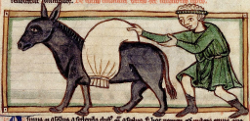
\includegraphics{asinus}}
        \caption{asinus, -ī (m)}
\end{figure}
Tulit ergō Moysēs uxōrem suam, et fīliōs suōs,
et imposuit eōs super asinum: reversusque est in Ægyptum,
portāns virgam Deī in manū suā. Dīxitque eī Dominus revertentī
in Ægyptum: ``Vidē ut omnia ostenta quæ posuī in manū tuā
\marginpar{indūrāre: durum facere}faciās cōram Pharaōne: ego indūrābō cor eius,
et nōn dīmittet populum. Dīcēsque ad eum: Hæc
\marginpar{prīmōgenitus: natū maior}dīcit Dominus: Fīlius meus prīmōgenitus Isrāēl.
Dīxī tibi: Dīmitte fīlium meum ut serviat mihi;
et nōluistī dīmittere eum:
ecce ego interficiam fīlium tuum prīmōgenitum.''

\marginpar{dīversōrium, -ī (n): aedificium in quō hominēs in itinere possunt dormīre}\marginpar{petra, -ae (f): lapis}Cumque esset in itinere, in dīversōriō
occurrit eī Dominus, et volēbat occīdere eum. 
\marginpar{idcircō: proptereā, ideō}Tulit idcircō Sephora acūtissimam petram,
\marginpar{praepūtium, -ī (n): illa pars puerī quae circumcīditur}et circumcīdit præpūtium fīliī suī, tetigitque pedēs ejus,
\marginpar{spōnsus/a: quī mox alicui maritus vel uxor erit}et ait: ``Spōnsus sanguinum tū mihi es.''
Et dīmīsit eum postquam dīxerat: ``Spōnsus sanguinum ob circumcīsiōnem.''

Dīxit autem Dominus ad Aarōn: ``Vāde in occursum Moȳsī
in dēsertum.'' 

Quī perrēxit obviam eī in montem Deī, et ōsculātus est eum.
Nārrāvitque Moysēs Aarōn omnia verba Dominī quibus miserat eum,
et signa quæ mandāverat. Vēnēruntque simul, et congregāvērunt
cūnctōs seniōrēs fīliōrum Isrāēl.
Locūtusque est Aarōn omnia verba quæ dīxerat Dominus ad Moysēn: et
fēcit signa cōram populō, et crēdidit populus.
Audiēruntque quod vīsitāsset Dominus fīliōs Isrāēl,
\marginpar{prōnus/a/um: iacēns in pectore}et respexisset afflīctiōnem illōrum: et prōnī adōrāvērunt.
